\section{Experiment 6}
Similar in structure to Experiment 1, this experiment aims to compare the results of a Gaussian classifier \code{fitcnb} and a k-Nearest Neighbours classifier. This experiment was conducted in an iterative manner, taking into account the average error across 10 iterations for each value of k and for each different sample size. These were then collated and compared to identify, at each value of sample size $N_{D}$, the lowest test error, the k-value corresponding to this, and the training error corresponding to that k-value. The k values in this iterative process needed to be limited to the total number of data-points $2N_{D}$. 


\subsection{Results \& Discussion}
Seen in Figure \ref{fig:Exp6} the k-value tended to be higher as $N_{D}$ increased, however this was also prone to variance in datasets and was not a monotonic effect. Ultimately this seems to perform marginally more effectively than the Gaussian classifier in Experiment 1. Comparing to Figure \ref{fig:Exp1} where the error tended to settle around an error of 0.2\%, the test set error with a k-Nearest Neighbour classifier seemed to settle at 0.13\% when comparing at $N_{D} = 100$, and with approximately 31-Nearest Neighbours being taken into account for the classification.

\begin{figure}[h]
	\centering
	\begin{subfigure}{.5\textwidth}
		\centering
		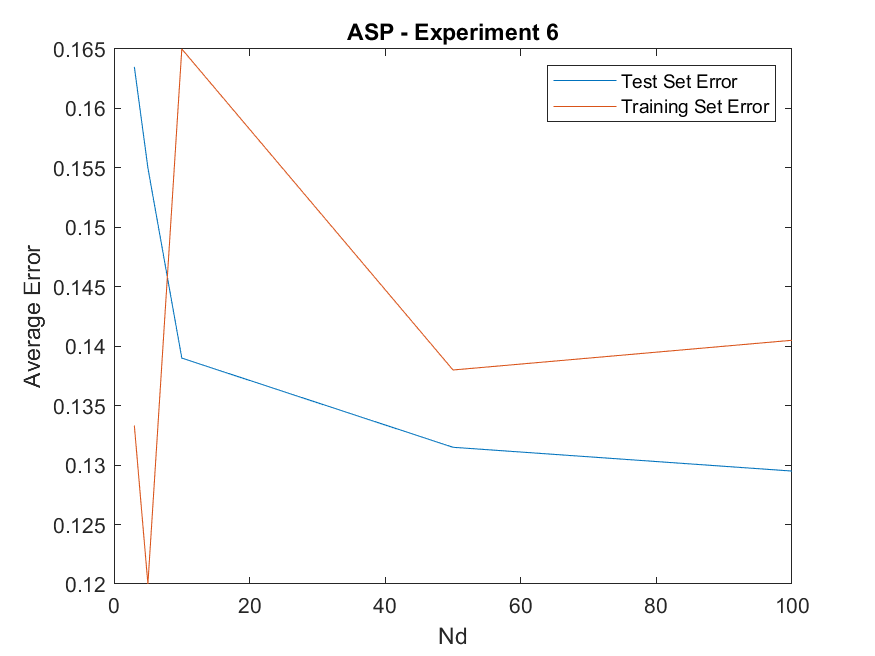
\includegraphics[width=.95\linewidth]{./code/Exp6-results/ErrorComparison.png}
		\caption{Lowest Error \% for k-Nearest Neighbour algorithm}
	\end{subfigure}%
	\begin{subfigure}{.5\textwidth}
		\centering
		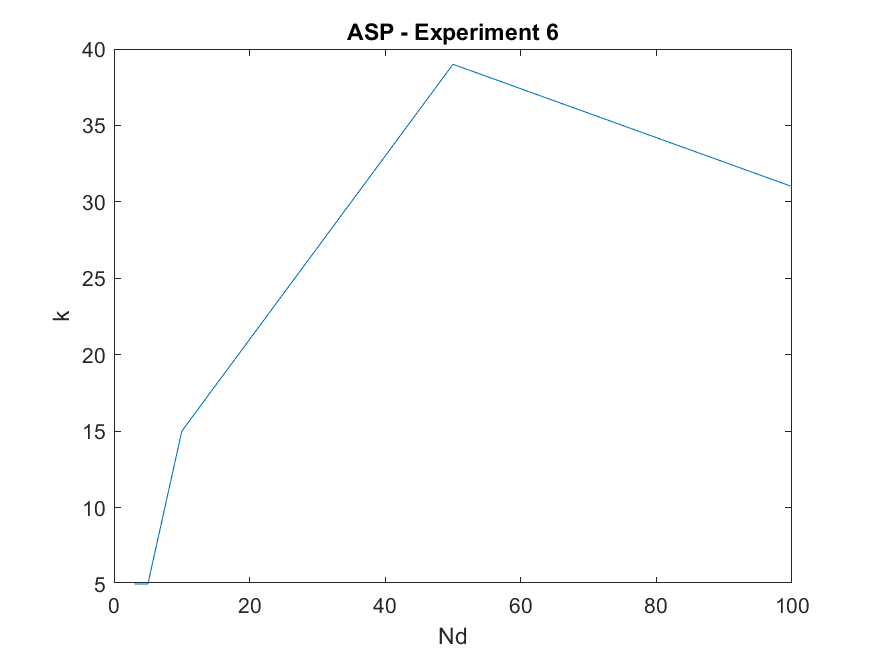
\includegraphics[width=.95\linewidth]{./code/Exp6-results/BestkVals.png}
		\caption{Optimum k value for k-Nearest Neighbour algorithm as a function of the size of the test dataset.}
	\end{subfigure}
	\caption{Experiment 6 Results - kNN comparison}
	\label{fig:Exp6}
\end{figure}

